\section{Experimental Setup}
\label{sec:experimentalsetup}

\subsection{Dataset and Point-in-Time Data Contract}
The daily universe spans information technology (FPT, CMG), banking (VCB, MBB), retail (MWG), food/beverages (VNM, BHN) and aviation/tourism (HVN, VJC). This is a purposive, non-representative sample: BHN, CMG, FPT, HVN, MBB, MWG, VCB, VJC and VNM. The reconstructed vnstock/VCI price snapshot \cite{vnstock_docs} covers observed vendor sessions from 2020 through September 2026. It is not an authenticated submission-time snapshot. Contradictory BHN OHLC data trigger the frozen valid-suffix policy; insufficient subsequent warm-up excludes BHN from three early blocks. No price is corrected to improve a result. This leaves 102 eligible cells of the 12-date by nine-symbol grid in Figure~\ref{fig:calendar}.

\paragraph{Two study identities}
We distinguish the original Full/Base revision study from the extension collection U08 and its frozen U09 analysis (editorial ID \texttt{unified\_u08\_u09\_r1}). They use the same eligible market calendar, but separate responses, method interfaces and provenance. Original-study Base omits both factor and sentiment sections; Common in the extension retains them under a different alpha/prompt profile. No original prediction is replaced by an extension prediction, and matching calendars do not justify a cross-study paired contrast or summed sample size. Sentiment is unavailable at \UnifiedMissingSentiment/\UnifiedPoints\ extension points; this remains missing input, not observed neutral sentiment.

\subsection{Walk-Forward Protocol}
Six blocks cover 2023 H2, 2024 H2, 2025 H1, 2025 Q4, 2026 Q2 and 2026 Q3, with two scheduled dates per block. These are twelve selected dates, not a continuous multi-year daily backtest; the chronological evaluation follows the walk-forward principle \cite{pardo2008evaluation} under this explicitly reduced schedule. Cross-symbol observations share calendar shocks. The 51 eligible symbol--block scopes contain chronological train/validation/test partitions: every train label exits before validation starts, and every validation label exits before the first test decision. Cutoffs require the frozen history length; label spans touching the next partition are purged.

The reduced scope was amended after some inference to complete a bounded historical study. Its 375 registered Decisions include 193 explicitly reused successful executions and 182 further successes. The factorial subset was selected by metadata (symbol/date round-robin), not prediction quality, but this does not make the overall amendment preregistered. The larger legacy grids remain incomplete/superseded. Table~\ref{tab:scope} distinguishes shared r0 calls, additional realizations and the separate factorial panel; their observations are not summed as independent markets.

\begin{figure}[!htb]
\centering
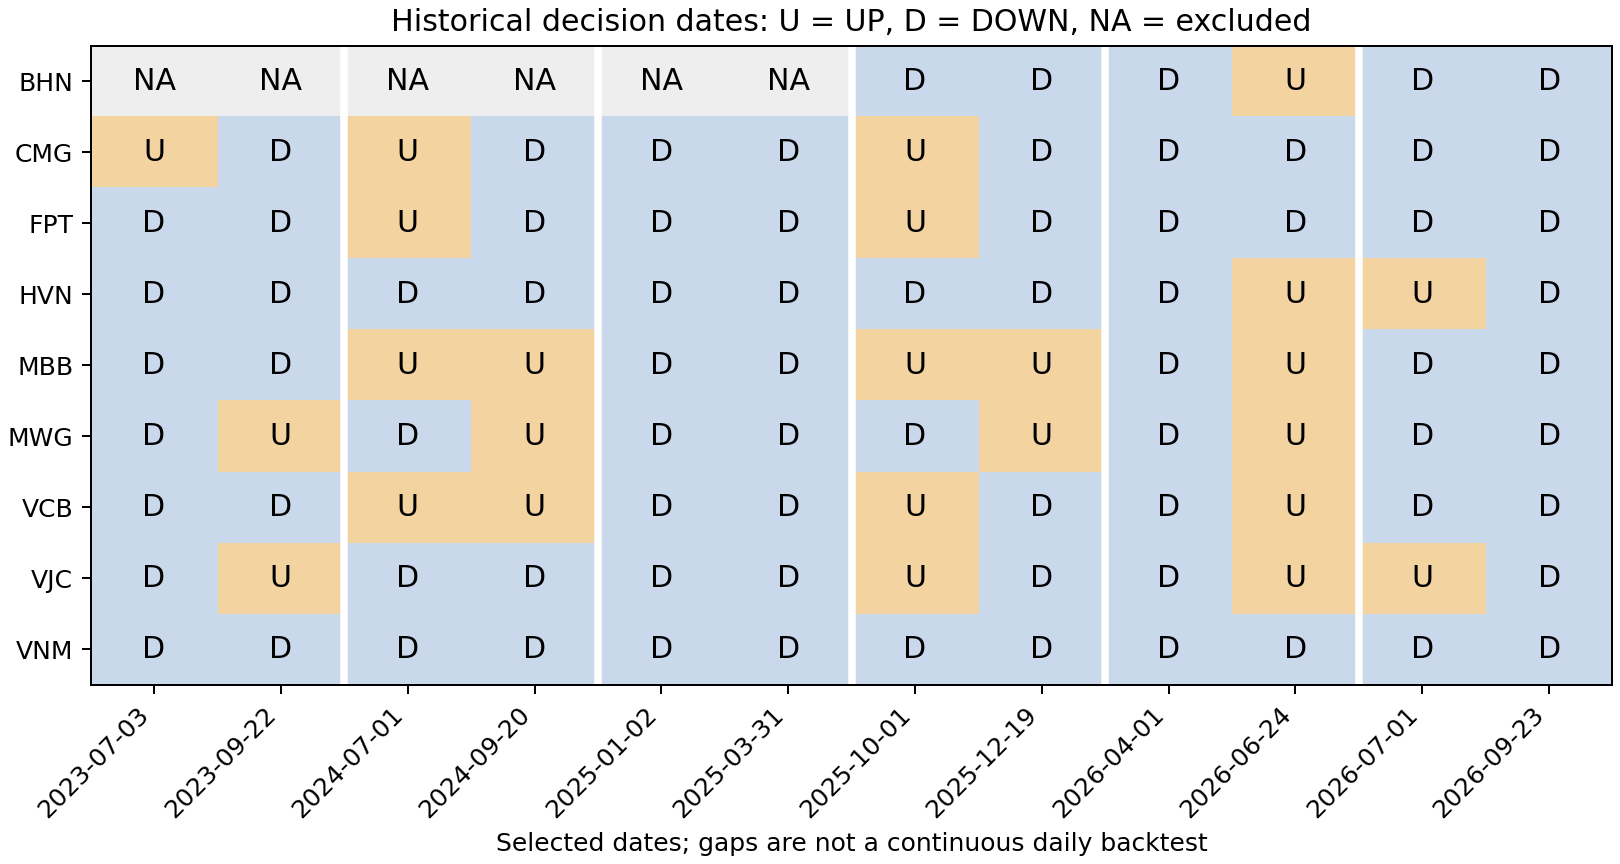
\includegraphics[width=\textwidth]{figs/final_calendar.png}
\caption{Historical decision dates and eligibility shared by the original and extension studies. Matching dates do not imply shared inference responses. Missing BHN cells remain excluded rather than being filled with CASH predictions. Labels are shared evaluation truth, not a visualization selected from Full's successful forecasts.}
\label{fig:calendar}
\end{figure}
\begin{table}[!htb]
\centering\small
\setlength{\tabcolsep}{3pt}
\renewcommand{\arraystretch}{1.15}
\caption{Evaluation scopes and prompt variants in the frozen historical study. Shared main/upstream executions are counted once.}
\label{tab:scope}
\textbf{A. Recorded supports}\par\smallskip
\begin{tabular}{lrrrrrrr}
\hline
Scope & $N$/exec. & Symbols & Dates & Blocks & UP/DOWN & Exec. & Decisions \\
\hline
Main & 102 & 9 & 12 & 6 & 25/77 & 1 & 204 \\
Upstream & 9 & 9 & 3 & 3 & 2/7 & 3 & 54 \\
Factorial & 9 & 8 & 4 & 3 & 2/7 & 3 & 135 \\
\hline
\end{tabular}\par\medskip
\textbf{B. Prompt sections}\par\smallskip
\begin{tabular}{llll}
\hline
Variant & Factors & Sentiment & Representation \\
\hline
B & -- & -- & Shared price reports \\
A & Current & -- & Five-row factorial \\
S & -- & Current & Factorial \\
AS & Current & Current & Compact main / five-row factorial \\
P & Past donor & Current & Five-row factorial \\
\hline
\end{tabular}\par\medskip
\begin{minipage}{\textwidth}\footnotesize Main uses B/AS; upstream uses B/AS; factorial uses B/A/S/AS/P. Class counts are per execution. Upstream includes 18 main r0 calls: 204+54+135-18=375 unique Decisions. P preserves current names/schema/missingness and sentiment, replacing factor values/signals/skill metadata by one past train-only rank-vector donor.\end{minipage}
\end{table}


The extension fixes \UnifiedPoints\ points, \UnifiedAccounts\ symbol--fold accounts, \UnifiedUpstreamRealizations\ upstream realization per point and \UnifiedDecisionRepeats\ Decision repeats. One immutable report/image parent is deep-copied into all roles; each repeat uses new Decision responses where a call is eligible. The \UnifiedForecastSlots\ research slots are not independent market samples, full-system executions or successful HTTP calls. All 102 evaluation IDs are reserved globally before context labels can be computed, including IDs belonging to earlier folds. Context is frozen before the first test query in a fold and reused at its second anchor; test labels are never added prequentially.
\begingroup
\let\savedscopepresentationtable\table
\def\table[#1]{\savedscopepresentationtable[!htbp]}
\begin{table}[!htb]
\centering\small
\setlength{\tabcolsep}{3pt}
\renewcommand{\arraystretch}{1.12}
\caption{Extension study U08/U09: distinct support and execution counts.}
\label{tab:u09-scope}
\textbf{Recorded support}\par\smallskip
\begin{tabular}{lr}
\hline
Quantity & Count \\
\hline
Market points & 102 \\
Symbols & 9 \\
Dates & 12 \\
Folds & 6 \\
Independent-capital accounts per repeat & 51 \\
Upstream realizations per point & 1 \\
Upstream executions & 102 \\
Points without available sentiment & 79 \\
Decision repeats & 3 \\
Research forecast slots (eight roles) & 2448 \\
Raw Decision responses & 1290 \\
HTTP attempts (including retired) & 1702 \\
\hline
\end{tabular}\par\medskip
\begin{minipage}{\textwidth}\footnotesize This study shares a test calendar with the original study, not its responses. Three Decision repeats do not add market observations or upstream realizations. BHN contributes six points in three recent folds; the other eight symbols contribute twelve each. Unavailable sentiment is missing input, not neutral news.\end{minipage}
\end{table}

\endgroup
% Không để bảng phạm vi trôi sang phần Results của bản submit.
\FloatBarrier

\begin{figure}[!htb]
\centering% Cutoff/context và hàng rào outcome; không đưa nhãn query vào prompt.
\begin{tikzpicture}[>=Latex,
 box/.style={draw=blue!55!black,fill=blue!4,rounded corners,align=center,text width=4.2cm,minimum height=1.45cm,font=\footnotesize},
 wide/.style={box,text width=15.4cm},arr/.style={->,thick}]
\draw[->,thick] (-0.3,0)--(14.5,0);
\draw[very thick,blue!60!black] (0,0.2)--(8.4,0.2);
\node[above,align=center,font=\footnotesize] at (4.2,0.3) {45-bar chart $[e-45,e)$\\Visible bars end at decision $d=e-1$};
\foreach \x/\lab in {0/{e-45},8.4/{d=e-1},10/{e},13.6/{e+2}}{\draw (\x,-0.12)--(\x,0.12);\node[below,font=\footnotesize] at (\x,-0.15) {$\lab$};}
\draw[<->,thick,orange!80!black] (10,1.4)--(13.6,1.4);
\node[above,align=center,font=\footnotesize] at (11.8,1.5) {Entry Open to exit Close\\$L=3$ observed bars};
\node[box] (train) at (2,-2.1) {\textbf{Chronological training}\\Fit orientation / scaler / teacher\\Labels mature before validation};
\node[box] (valid) at (7.1,-2.1) {\textbf{Purged validation}\\Select before the test fold\\Freeze resources / checkpoint};
\node[box] (test) at (12.2,-2.1) {\textbf{Held test schedule}\\Twelve dates / six folds\\BHN early cells excluded};
\draw[arr] (train)--(valid);\draw[arr] (valid)--(test);
\node[wide] (context) at (7.1,-4.4) {\textbf{Point-in-time preparation before each query}\\Prior cycles: exit $<d$; dated news only through $d$; prefix-only regime filtering.\\Context is frozen before the fold's first query; exclude all 102 evaluation IDs.\\Frozen train/validation resources are not fitted again on queries or repeats.};
\draw[arr] (test.south)--(test.south |- context.north);
\node[wide] (shared) at (7.1,-6.9) {\textbf{One shared upstream realization at the point}\\Freeze I/P/T reports and exact charts; bind native/common alpha projections.\\Deep-copy the same parent to all roles and all three extension Decision repeats.};
\draw[arr] (context)--(shared);
\node[wide] (decision) at (7.1,-9.2) {\textbf{Dependency-ordered Decisions within each repeat}\\Common $\rightarrow$ priors / fact anchor; Common + anchor $\rightarrow$ MT revision.\\Persist raw proposal, policy action, bypass reason and provenance; checkpoint / retry.};
\draw[arr] (shared)--(decision);
\node[wide,fill=orange!7] (out) at (7.1,-11.5) {\textbf{Outcome barrier after every required forecast is durable}\\Join immutable net truth; LONG: Open$(e)$ to Close$(e+2)$; SHORT: CASH.\\Separate account per symbol/fold/repeat; no evaluation label feeds back into context.};
\draw[arr] (decision)--(out);
\end{tikzpicture}

\caption{Walk-forward timing, frozen resources and forecast/outcome barrier. The chart ends at $d=e-1$, entry is at $e$ and the $L=3$ target is at $e+2$: equivalently Open$(t+1)$ to Close$(t+3)$. Prior exits precede the cutoff and all evaluation IDs stay outside context. The extension uses one upstream realization and three Decision repeats per point on twelve selected dates/six folds, not a uniform $S=3$ grid. Outer cutoff isolation does not certify native row-wise causality.}
\label{fig:walkforward}
\end{figure}

\subsection{Paired Baseline and Disentangled Ablations}
All nine classifiers use the same 102 main units and net target. CASH and always-LONG are constant predictions; always-LONG closes and pays costs every cycle. Train-majority uses purged training labels, choosing CASH on a tie. Momentum predicts LONG for a strictly positive trailing 20-session return. The logistic comparators use scikit-learn \cite{pedregosa2011sklearn}. Logistic-price uses numerical price features; logistic-matched adds the recorded factor/sentiment/missingness inputs. Imputation, scaling, regularization and decision threshold selection follow chronological train/validation rules; final logistic refits use matured train plus validation only. We reuse their saved predictions rather than refitting after observing outcomes. The fixed factor-vote comparator uses training-fitted medians/orientation and differs from the native top-five policy and the auxiliary numeric-control study.

Matched numerical inputs do not equal chart images, report wording or pretrained knowledge. Full--Base differences likewise include prompt structure, report length and propensity to choose CASH. The upstream panel has nine units, B/AS and three regenerated upstream realizations with a Decision execution per realization. The factorial panel has nine different-support units, B/A/S/AS/P and three Decision executions with fixed upstream. Both have two UP/seven DOWN per execution, but only the former covers nine symbols. We do not infer main-grid variability or separate upstream/Decision variance components from their SDs.

P retains current factor names, headings, schema/missingness and sentiment, replacing scalar values, signals and skill fields using a predetermined earlier train-only rank-vector donor. Donor label exits precede validation/test. Rank mapping is not name-matched covariance preservation, a placebo distribution or exposure matching. Five explicit rows reach each A/AS/P factorial prompt. Main/upstream compact prompts are a separate representation family. Interaction is defined as $AS-A-S+B$; the observed best-single gap $AS-\max(A,S)$ is a different, post-hoc diagnostic and not an eighth factorial contrast.

\paragraph{Extension baselines and dependencies}
The extension evaluates Native, Common, five extensions, Fact\_Anchor and two no-LLM controls, CASH and Always-LONG cycles with full costs. Five extensions are compared separately with Native (system family) and Common (method family). Fact\_Anchor is a dependency/control, not a sixth claimed improvement. Three descriptive bridges compare Common with Native, Fact\_Anchor with Common, and MT-BICL with Fact\_Anchor. Neither these bridges nor economic controls enter the primary contrast family. The original nine-unit upstream/factorial panels above remain evidence for their own interventions; new retrieval/content/MT ablations were not executed in U08/U09.

\subsection{Account and Statistical Metrics}
BA averages UP and DOWN recall \cite{brodersen2010balanced}; MCC \cite{chicco2020mcc} and both-class precision/recall accompany ordinary accuracy and LONG rate. Pooled metrics retain actual class supports. Symbol macro means are unweighted and report planned/defined denominators. Missing class support or a degenerate MCC denominator yields NA, not zero. Following dependent-data resampling principles \cite{lahiri2003resampling}, main contrasts use 10,000 paired whole-block resamples, seed 20261102, retaining dates, cross-section, variants and eligibility together. Repeat diagnostics jointly resample recorded blocks and paired execution indices. Intervals condition on finite draws; undefined counts remain visible. Circular block lengths, leave-one-block-out and Bartlett HAC \cite{newey1987hac} at lags 0/1/2 are sensitivity diagnostics. HAC uses calendar-aligned accuracy differences in fixed-universe panels, with a $t(n_{dates}-1)$ reference; few clusters, irregular gaps and post-inference additions prevent calibrated significance or power claims.

To specify the classification estimand, let TP/FN count UP outcomes and TN/FP count DOWN outcomes. We use
\begin{equation}
 \begin{aligned}
 BA&=\frac12\left(\frac{TP}{TP+FN}+\frac{TN}{TN+FP}\right),\\
 MCC&=\frac{TP\,TN-FP\,FN}{\sqrt{(TP+FP)(TP+FN)(TN+FP)(TN+FN)}}.
 \end{aligned}
 \label{eq:classification_metrics}
\end{equation}
The relevant metric is undefined when a required denominator is zero. Macro means average defined symbol-level values while retaining the planned and defined denominators. A CASH rule can have high ordinary accuracy in a DOWN-heavy sample without discriminating the two classes.

Each of 51 symbol--block accounts starts with VND50 million, without cross-symbol capital competition. LONG follows Eq.~\ref{eq:label}; CASH stays flat. Continuous hold buys once from the first entry through the last scheduled exit, including gaps, and is not a tenth classifier. Wealth includes pending receivables and residual shares at recorded mark-to-market prices. Daily-close drawdown uses an initial-capital anchor. Where supplied in companions, daily Sharpe uses population SD and a 252-session convention with zero risk-free rate; the retained Sortino convention uses SD of negative daily observations, not downside RMS. Downside-risk ratios \cite{sortino1994downside} depend on this denominator choice, so these conventions are kept explicit. Annualised cycle ratios are NA for the irregular/gapped main schedules, and are not presented as investment-quality estimates from a handful of trades.

The reference assumes fractional fills at recorded prices and two-leg fees/slippage. Shares are assumed sellable in the afternoon of T+2 conditional on allocation and fill; sale proceeds are pending until the specified settlement phase. This convention follows the archived settlement source \cite{vsd2022settlement}. L=3 is a fixed observed-bar protocol choice, not an optimized horizon. Daily OHLC cannot authenticate opening-auction queues, price-limit fills, partial fills or correct volume units. All twelve sensitivities, including pending cash, advances, cost changes, sell charge, no-fill/delay proxies and lot/capacity assumptions, remain in \ref{app:additional}. Venue/calendar review flags, including ten HVN unit flags, are retained rather than converted to certified fills or synthetic CASH.

\paragraph{Extension estimands and uncertainty}
For U09, each role has three independent-capital executions per symbol--fold account. Account returns are averaged across repeats within account, then equally over 51 accounts; BA is computed on the 102 points separately per repeat and then averaged. Final policy actions determine the evaluated prediction, while raw proposals remain available. Daily EOD NAV, cycle-end drawdown, fees/slippage, turnover and held-session fraction retain their separate units. The extension's cycle Sharpe uses sample SD (ddof=1) and its cycle Sortino uses the RMS of negative-part returns over all cycles with MAR zero. These are different conventions from the original study's daily ratios above. Annualized ratios remain null; a degenerate denominator or missing class stays null/NA with its reason.

The extension uses paired circular fold bootstrap draws with block length two, 10,000 draws, PCG64 seed 20261110, retaining cross-section, eligibility and all methods/repeats together. Identical resample indices serve all twenty return/BA endpoint contrasts in the two registered families. Simultaneous descriptive bands use standardized maximum deviation across those twenty columns. Finite/null rules apply jointly; draws are not redrawn to hide an undefined endpoint, and a degenerate family does not receive substitute bands. L1/L3, leave-one-fold-out, leave-one-symbol-out and the fixed CORE4 subset remain sensitivity analyses. These six historically exposed folds do not establish calibrated coverage, significance or power. The original-study seed, estimands and finite-draw conventions remain unchanged.

\subsection{Implementation and Robustness Design}
Archived SDK aliases are \texttt{openai/gpt-oss-20b} for text and \texttt{qwen/qwen3.8-27b} for vision. Configured temperature zero appears as $10^{-8}$ in observed SDK metadata; no hosted decoding seed is recorded. Text/vision output caps are 2,048/1,024 tokens. Retry/checkpoint records preserve individual attempts and completed outputs. Aliases and 40 response fingerprints do not authenticate an immutable weight revision or historical provider catalogue; 91 original Pattern requests lack epoch/provider-org fields and remain unknown. Offline replay reproduces saved-prediction metrics, not a fresh hosted inference experiment.

The closure contains 649 attempts, 615 successes and 34 errors, including 120 original Pattern calls replayed as shared dependencies. Observed usage totals 1,063,328 prompt and 340,736 completion tokens. Error usage/latency and monetary billing are unknown. Pattern tokens/latency describe original calls, not replay lookup cost; successful callback elapsed times are not wall-clock runtime. Full accounting, pins and hashes are in repository artifacts rather than an implementation appendix.

\paragraph{Frozen extension resources and attempts}
U08 locks its own observed SDK options, prompts and aliases rather than assuming that the original-study responses were reused. It retains the text/vision aliases named above, temperature and output-cap metadata, one retry owner, durable request intents and intermediate checkpoints. Three total attempts include schema repair; an UNKNOWN request is reserved and reconciled instead of blindly resent. Dependency order constrains counterbalancing, and actual branch/repeat/provider order remains in the ledger. The sealed ledger has 1,702 HTTP attempts including 15 retired raw records retained after authorized resets, while the active grid has 1,290 raw Decision responses. These counts describe different objects and are not added to the original closure's 649 attempts. The maximum successful/repaired Decision request length is recorded in the U08 acceptance, not inferred from the original profile.

The prior bank contains 852 frozen CORE4 tasks (FPT/MWG/VCB/VNM) from its own raw execution lineage; OOD5 uses declared support/fallback rather than fabricated same-symbol examples. The compatibility audit found numeric net-return differences between donor/raw and canonical query construction in 828/852 records, with maximum absolute discrepancy about 0.042988489 percentage points; this is not a count of binary label flips. The raw bank is retained without relabeling it as causal-common history. Numeric MT context, scaler, HMM and teacher are frozen with the selected student checkpoint (seed 42, step 3000); inference performs forward evaluation only. All 51 causal alpha selector bindings precede their queries. \ref{app:software} identifies the manifests needed to audit these resources and the source bridge.
